%% LyX 2.1.4 created this file.  For more info, see http://www.lyx.org/.
%% Do not edit unless you really know what you are doing.
\documentclass[unicode,pdfcover]{sufethesis}
\usepackage{fontspec}
\usepackage{color}
\usepackage{array}
\usepackage{longtable}
\usepackage{graphicx}
\usepackage[unicode=true,
 bookmarks=true,bookmarksnumbered=true,bookmarksopen=false,
 breaklinks=false,pdfborder={0 0 1},backref=false,colorlinks=true]
 {hyperref}
\hypersetup{pdftitle={事件抽取技术研究综述},
 pdfauthor={王华杰},
 pdfsubject={上海财经大学博士学位论文论述},
 pdfkeywords={关键字1, 关键字2},
 unicode=false,linkcolor=blue, anchorcolor=black, citecolor=olive, filecolor=magenta, menucolor=red, urlcolor=magenta, pdfstartview=FitH}

\makeatletter

%%%%%%%%%%%%%%%%%%%%%%%%%%%%%% LyX specific LaTeX commands.
\providecommand{\LyX}{\texorpdfstring%
  {L\kern-.1667em\lower.25em\hbox{Y}\kern-.125emX\@}
  {LyX}}
%% Because html converters don't know tabularnewline
\providecommand{\tabularnewline}{\\}

\makeatother

\usepackage{xunicode}
\begin{document}

\title{上海财经大学博士毕业论文}


\author{王华杰}


\supervisor{指导教师:王英林\ 教授}


\institute{上海财经大学}


\date{2017年11月28日}

\maketitle
\frontmatter
% 2017-11-28 basilwang 暂时去掉英文摘要
%
%\begin{abstractCN}
%本文主要介绍了上海财经大学博士学位论文\LaTeX 和\LyX{}模板的使用方法。本模板根据华南理工大学博士学位论文\href{https://github.com/alwintsui/scutthesis}{模板}修改制作而成,在此表示感谢。
%\end{abstractCN}
%
%\keywordsCN{\textbf{毕业论文;上海财经大学;\textbf{\LaTeX};\LyX{}}}
%\begin{abstractEN}
%The english abstract.
%\end{abstractEN}

% 2017-11-28 basilwang 暂时去掉关键字
%\keywordsEN{\textbf{Thesis; SUFE; \textbf{\LaTeX}; \LyX{}}}

\tableofcontents{}

\mainmatter


\chapter{选题背景、理论意义、实用价值}


\section{背景、理论意义}


\section{实用价值}

\subsection{实用价值1} 

基础模板来源于华南理工大学博士学位论文\href{https://github.com/alwintsui/scutthesis}{模板},并根据上海财经大学学位论文的要求进行了相应的修改。

\subsection{实用价值2}

基础模板来源于华南理工大学博士学位论文\href{https://github.com/alwintsui/scutthesis}{模板},并根据上海财经大学学位论文的要求进行了相应的修改。


\chapter{文献综述}


\section{国内外研究现状}

基础模板来源于华南理工大学博士学位论文\href{https://github.com/alwintsui/scutthesis}{模板},并根据上海财经大学学位论文的要求进行了相应的修改。


\subsection{国内外研究现状1}

基础模板来源于华南理工大学博士学位论文\href{https://github.com/alwintsui/scutthesis}{模板},并根据上海财经大学学位论文的要求进行了相应的修改。
\subsection{国内外研究现状2}

基础模板来源于华南理工大学博士学位论文\href{https://github.com/alwintsui/scutthesis}{模板},并根据上海财经大学学位论文的要求进行了相应的修改。

\section{发展趋势}


基础模板来源于华南理工大学博士学位论文\href{https://github.com/alwintsui/scutthesis}{模板},并根据上海财经大学学位论文的要求进行了相应的修改。

%\subsection{事件抽取面临的挑战}
%大量关于事件抽取的研究,使得事件抽取在理论和应用方面都取得了长足的进步。但是从ACE等评测会议的评测结果来看,目前事件抽取的精度远未到达实际应用的要求,大多在70\%左右,研究发展依然面临诸多挑战。
%
%1)	底层技术研究不够成熟,导致错误级联。事件抽取对底层的子任务结果有很大的依赖性,但由于实体识别、深层句法分析等底层技术还不成熟,给事件抽取带来了级联错误。并且,目前缺乏对子任务输出结果的评估及矫正技术。
%
%2)	事件抽取系统的领域可扩展性和可移植性不够理想。目前的研究大多是基于MUC或ACE展开,只针对某个特定领域或几个类型的时间进行研究。系统的应用受到领域的限制,不能随着领域的变化进行简单快速的移植或扩展。
%
%3)  语料有待进一步完善。机器学习方法的引入提高了事件抽取系统的可移植性,但由于缺乏大规模的成熟语料库和标准语料,目前该类系统的效果不够理想,由此可见语料的完善是一个亟待解决的问题。
%\subsection{事件抽取的研究趋势}
%尽管面临诸多挑战,但事件抽取的研究必将受到学者越来越多的而关注,并在未来的研究中呈现出一下趋势。
%
%1)	进一步提高时间抽取的精度和召回率,改进抽取的方法,加强底层技术攻关,开展对中间结果的可信度评估研究。要使时间抽取技术取得突破,必须改进其所依赖的底层技术。
%
%2)	跨文档、跨语言的事件抽取研究将更为广泛。目前,事件抽取的水平还局限在对独立文本的处理上,跨文档的研究尚处于探索阶段,随着跨文档语义理解及信息归并技术和多语言文本处理技术的发展,跨文档、跨语言的事件抽取必然成为新的研究热点。
%
%3)	面向开放领域的事件抽取将广受重视。事件抽取系统的领域可扩展性和可移植性仍将是研究的重点。未来的事件抽取研究将以应用为需求,面向开放领域而不再局限于某个具体领域,为此需要探究各种方式提高系统的移植性。

\chapter{研究的基本思路与方法}

\section{研究思路}

基础模板来源于华南理工大学博士学位论文\href{https://github.com/alwintsui/scutthesis}{模板},并根据上海财经大学学位论文的要求进行了相应的修改。



\section{研究方法}

基础模板来源于华南理工大学博士学位论文\href{https://github.com/alwintsui/scutthesis}{模板},并根据上海财经大学学位论文的要求进行了相应的修改。

\chapter{论文的创新性尝试}

基础模板来源于华南理工大学博士学位论文\href{https://github.com/alwintsui/scutthesis}{模板},并根据上海财经大学学位论文的要求进行了相应的修改。




\chapter{研究难点与预期成果}

研究难点:

基础模板来源于华南理工大学博士学位论文\href{https://github.com/alwintsui/scutthesis}{模板},并根据上海财经大学学位论文的要求进行了相应的修改。
预期成果:

基础模板来源于华南理工大学博士学位论文\href{https://github.com/alwintsui/scutthesis}{模板},并根据上海财经大学学位论文的要求进行了相应的修改。

\chapter{研究范围与目前进展情况}

研究范围: 本文拟分为6章,章节目安排如下:
1. 绪论

1.1 背景

1.2 研究意义

1.3 研究内容

1.4 研究方法和技术路线

1.5 创新点和章节安排

2. 文献综述

2.1 相关概念界定

2.2 国内外文献综述

2.2.1 元事件抽取

2.2.2 主题事件抽取

2.3 相关理论

2.4 文献评述

2.5 小结

3. 

3.1 引言
 
3.2 相关工作
 
3.3 
 
3.4 

3.5 

3.6 实验
  
3.7 小结
   
4. 
   
4.1 引言
   
4.2 相关工作
   
4.2.1 
   
4.2.2 
   
4.3 
   
4.4 
   
4.4.1 
   
4.4.2 
   
4.5 
   
4.5.1 

4.5.2 

4.6 实验

4.6.1 实验数据

4.6.2 事件抽取实验

4.6.3 事件表示实验
   
5. 
   
5.1 引言
    
5.2 相关工作
    
5.3 
    
5.3.1 

5.3.2 

5.3.3 
    
5.4 特征表示
    
5.5 实验

5.5.1 实验数据

5.5.2 评价方法

5.5.3 基线方法

5.5.4 实验结果与分析

5.6 本章小结
     
6. 总结与展望
      
6.1 研究结论
      
6.2 研究展望


\chapter{论文写作进度时间安排}

2017 年 11-12 月 完成绪论

2018 年  1- 4 月 完成论文第二章(文献综述和数据收集任务) 

2018 年  4- 8 月 完成论文第三章

2018 年  8- 12 月 完成论文第四章

2019 年  1- 4 月 完成论文第五章

2019 年  5-6 月 完成总结与展望及论文全文,论文定稿

   

\chapter{使用方法}


\section{基本使用方法}

对于\LaTeX{}用户,请使用根目录下的Thesis\_main.tex相应修改即可,并使用xelatex命令进行编译。对于\LyX{}用户,修改Thesis\_main.lyx即可。


\section{格式修改需求}

格式定义在sufethesis.cls文件中,可以根据自己的需求修改此文件。在不确定的情况下不建议直接修改此文件。


\section{字体}

本模板在mac下编译通过,如果使用其他系统(如Linux、Windows等),需要修改sufethesis.cls中的字体为相应的系统字体:
\begin{quotation}
\textbackslash{}setCJKmainfont\{Songti SC\}

\textbackslash{}setCJKfamilyfont\{song\}\{Songti SC\}

\textbackslash{}setCJKfamilyfont\{hei\}\{Heiti SC\} 

\textbackslash{}setCJKfamilyfont\{kai\}\{Kaiti SC\} 

\textbackslash{}setCJKfamilyfont\{fang\}\{STFangsong\}

\textbackslash{}newcommand\{\textbackslash{}songti\}\{\textbackslash{}CJKfamily\{song\}\} 

\textbackslash{}newcommand\{\textbackslash{}heiti\}\{\textbackslash{}CJKfamily\{hei\}\} 

\textbackslash{}newcommand\{\textbackslash{}kaiti\}\{\textbackslash{}CJKfamily\{kai\}\} 

\textbackslash{}newcommand\{\textbackslash{}fangsong\}\{\textbackslash{}CJKfamily\{fang\}\}
\end{quotation}
将「Songti SC」等分别修改为系统对应的字体即可。\textbf{不修改字体会导致编译不通过}。


\section{公式录入}

公式输入与\LaTeX{}及\LyX{}使用方法一致,如$y=x'\beta+\epsilon$,以及:
\[
\hat{\beta}=\left(X'X\right)^{-1}X'Y
\]
此外公式可以进行编号:
\begin{equation}
\hat{\beta}_{iv}=\left[X'Z\left(Z'Z\right)^{-1}Z'X\right]^{-1}\left[X'Z\left(Z'Z\right)^{-1}Z'Y\right]
\end{equation}
公式编号自动按照章进行分组。


\section{定理声明}

可以声明定理等,如:
\begin{theorem}
OLS估计为最优无偏线性估计量(BLUE),且$\hat{\beta}\overset{p}{\rightarrow}\beta$。\end{theorem}
\begin{proof}
略。
\end{proof}


\section{图片、表格插入}

图片和表格编号实例:

\begin{table}


\caption{表格示例}


\begin{centering}
\begin{tabular}{ccc}
\hline 
 & (1) & (2)\tabularnewline
\hline 
labor & $\underset{(0.2)}{0.7}${*}{*} & $\underset{(0.2)}{0.7}${*}{*}\tabularnewline
capital & $\underset{(0.1)}{0.3}${*}{*} & $\underset{(0.1)}{0.3}${*}{*}\tabularnewline
Constant & $\underset{(0.5)}{1.5}${*}{*} & $\underset{(0.5)}{1.5}${*}{*}\tabularnewline
\hline 
\multicolumn{3}{l}{{\small{}注:仅为示意性展示}}\tabularnewline
\hline 
\end{tabular}
\par\end{centering}

\end{table}


\begin{figure}
\begin{centering}
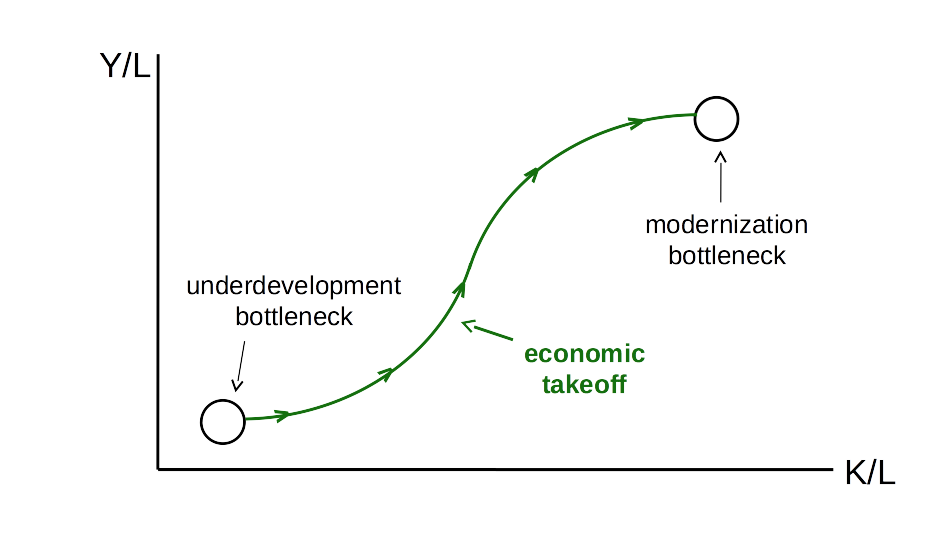
\includegraphics[scale=0.4]{figures/1}
\par\end{centering}

\caption{图示例}


\end{figure}



\section{参考文献}

参考文献可以使用Bib\TeX{}进行管理,覆盖sufethesis.bib即可。





%\chapter{总结与展望}
%
%综上所述,国内外学者以对事件抽取技术进行了较多的研究,取得了一些理论和应用上的成果,但事件抽取技术仍未到达实际应用的水平。目前,制约事件抽取技术广泛应用的两个最主要的因素是系统性能和可移植行。今后的研究将紧紧围绕如何克服和解决这两个问题展开,不断提高事件抽取系统的性能,增强其可移植性。
%
%在情报研究工作中,事件抽取技术的应用解决了如何快速准确地从海量信息集合中提取出用户感兴趣的事件的问题,将由人工阅读提取的过程转化成计算机的自动提取,能极大地提高工作效率,为信息服务向知识服务转型提供支撑技术。在情报研究领域事件抽取技术的应用研究较少,缺乏相应的应用系统,基于事件抽取技术构建相关情报研究支持系统具有广阔的应用前景和巨大的现实意义。




% 2017-11-28 basilwang 暂时去掉
%\chapter{参考文献}
%
%参考文献可以使用Bib\TeX{}进行管理,覆盖sufethesis.bib即可。

% 2017-11-28 basilwang 暂时去掉结论
%\chapter{结论}
%Enjoy it.

\bibliographystyle{sufethesis}
\nocite{*}
\bibliography{sufethesis}


% 2017-11-28 basilwang 暂时去掉致谢
%\chapterx{致谢}
%
%感谢之前的代码提供者,特别是华南理工大学博士学位论文\href{https://github.com/alwintsui/scutthesis}{模板}的制作者。

% 2017-11-28 basilwang 暂时去掉署名
%\begin{minipage}[t]{0.8\columnwidth}%
%\begin{flushright}
%王华杰
%\par\end{flushright}
%
%\begin{flushright}
%2017年11月28日
%\par\end{flushright}%
%\end{minipage}


% 2017-11-28 basilwang 暂时去掉研究成果

%\chapterx{攻读博士学位期间取得的研究成果}
%
%已发表(包括已接受待发表)的论文,以及已投稿、或已成文打算投稿、或拟成文投稿的论文情况(只填写与学位论文内容相关的部分):

%\begin{table}
%\begin{longtable}{|>{\centering}m{0.5cm}|>{\centering}m{2.3cm}|>{\centering}m{3.5cm}|>{\centering}m{2.6cm}|>{\centering}m{2cm}|>{\centering}m{1.3cm}|>{\centering}m{0.9cm}|}
%\hline 
%序号 & 作者(全体作者,按顺序排列) & 题 目 & 发表或投稿刊物名称、级别 & 发表的卷期、年月、页码 & 相当于学位论文的哪一部分(章、节) & 被索引收录情况\tabularnewline
%\hline 
%1 &  &  &  &  &  & \tabularnewline
%\hline 
% &  &  &  &  &  & \tabularnewline
%\hline 
% &  &  &  &  &  & \tabularnewline
%\hline 
% &  &  &  &  &  & \tabularnewline
%\hline 
% &  &  &  &  &  & \tabularnewline
%\hline 
% &  &  &  &  &  & \tabularnewline
%\hline 
%\end{longtable}
%\end{table}

\end{document}
